\section{Positive or negative}
\subsection{Aim}
To check whether the given number is positive or negative

\subsection{Code}
\begin{lstlisting}
; To check whether the given number is positive or negative.

ORG 0000H

; Resetting R0
MOV R0, #00H
; Number to check whether positive or negative
MOV R1, #0FFH
; Rotating the number, MSB goes to carry
MOV A, R1
RLC A
JC NEG ; Jump to NEG if carry flag is set
MOV R0, #0H
JMP EXIT

NEG:
	MOV R0, #1H

EXIT:
	NOP

END
\end{lstlisting}

\subsection{Output}
\textbf{Input} 0FFH (R1)\\
\textbf{Output} 01 (R0) (01 implies it is negative)\\
\begin{center}
	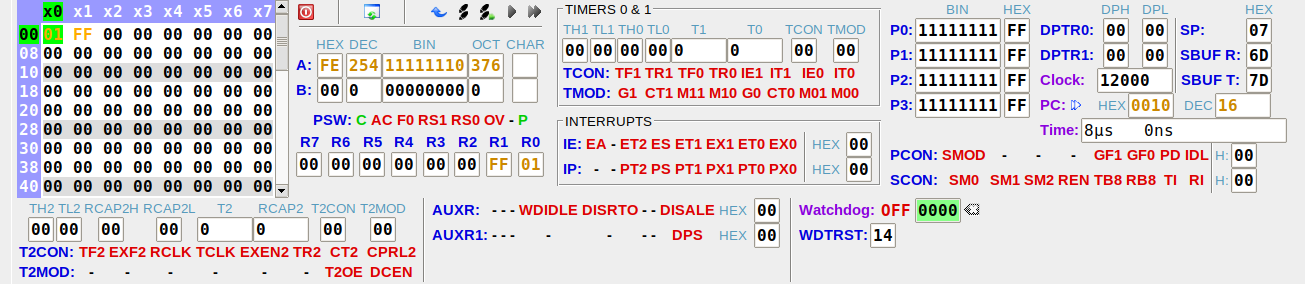
\includegraphics[width=\textwidth]{img/p24/ss1.png}
	\newline
\end{center}

\textbf{Input} 00FH (R1)\\
\textbf{Output} 00 (R0) (00 implies it is positive)\\
\begin{center}
	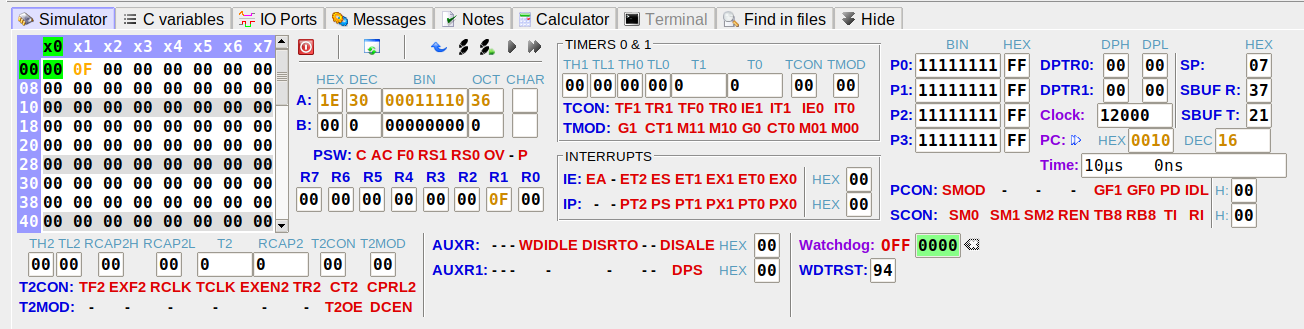
\includegraphics[width=\textwidth]{img/p24/ss2.png}
\end{center}

\subsection{Result}
A number was checked to be whether positive or negative in mcu8051ide